\chapter{Analisi Sintattica}
$S \rightarrow cAd$\\
$A \rightarrow ab | a$\\

%%%%%%%%%%%%%%%%%%%%%%%%%%%%%%%%%%%%%%%%%%%%%%%%%%%%%%%%%%%%%%%%%%%%%%%%%%%%%%%%%%%%%%%%%%%%%%%%
\section{Parsing Top-down}
Parto dal starting symbol ed espando le derivazioni dando priorit\'a alle derivazioni pi\'u a sinistra.
Cerco quindi di ricostruire una derivazione leftmost della stringa w data in input.\\[5pt]
$w\$, \$ \not\in V$\\
$w=cabd$\\[5pt]
Per ricostruire la parola w parto dalla prima derivazione $S \rightarrow cAd$ derivo la A pi\'u a sinistra (leftmost) e posso scegliere 
fra $a$ ed $ab$; scelgo $a$ e mi accorgo che ho sbagliato, torno in dietro e scelgo $ab$.

%%%%%%%%%%%%%%%%%%%%%%%%%%%%%%%%%%%%%%%%%%%%%%%%%%%%%%%%%%%%%%%%%%%%%%%%%%%%%%%%%%%%%%%%%%%%%%%%
\section{Parsing Top-down predittivo (o non ricorsivo)}
Cambio la grammatica sopra in: \\
$S \rightarrow cAd$\\
$A \rightarrow aB$\\
$B \rightarrow b | \varepsilon $\\[5pt]
$S \rightarrow cAd \rightarrow caBd \rightarrow \text{vedo che mi serve una b, escludo a priori } \varepsilon$\\ 

%%%%%%%%%%%%%%%%%%%%%%%%%%%%%%%%%%%%%%%%%%%%%%%%%%%%%%%%%%%%%%%%%%%%%%%%%%%%%%%%%%%%%%%%%%%%%%%%
\section{Grammatica LL(1)}
Le grammatiche LL(1) sono un subset delle grammatiche libere.\\
\begin{tabular}{cl}
    prima \textbf{L}    & leggiamo la input string da sinistra (left)\\
    seconda \textbf{L}  & ricostruiamo una leftmost derivazione\\
    \textbf{(1)}        & decidiamo quale operazione effettuare guardando un solo simbolo in input\\
\end{tabular}


%%%%%%%%%%%%%%%%%%%%%%%%%%%%%%%%%%%%%%%%%%%%%%%%%%%%%%%%%%%%%%%%%%%%%%%%%%%%%%%%%%%%%%%%%%%%%%%%
\section{First}
Data una generica $\alpha \in V^*$ per G=(V, T, S, P), first($\alpha$) \'e l'insieme dei simboli terminali b tali che $\alpha \implies bv$.
Inoltre se $\alpha \implies \varepsilon $ allora $\varepsilon \in first(\alpha )$

%%%%%%%%%%%%%%%%%%%%%%%%%%%%%%%%%%%%%%%%%%%%%%%%%%%%%%%%%%%%%%%%%%%%%%%%%%%%%%%%%%%%%%%%%%%%%%%%
\subsection{Esercizio}
$S \rightarrow A|B$\\
$A \rightarrow a|C$\\
$C \rightarrow \varepsilon$\\
Allora first(A) = $\{ a, \varepsilon \}$ ($\varepsilon$ perch\'e posso fare $A \implies C \implies \varepsilon $). 

%%%%%%%%%%%%%%%%%%%%%%%%%%%%%%%%%%%%%%%%%%%%%%%%%%%%%%%%%%%%%%%%%%%%%%%%%%%%%%%%%%%%%%%%%%%%%%%%
\subsection{Esercizio}
$S \rightarrow A|B$\\
$A \rightarrow a|C$\\
$C \rightarrow bB$\\
Allora first(A) = $\{ a, b \}$ (b perch\'e posso fare $A \implies C \implies bB$, ma B non esiste). 

%%%%%%%%%%%%%%%%%%%%%%%%%%%%%%%%%%%%%%%%%%%%%%%%%%%%%%%%%%%%%%%%%%%%%%%%%%%%%%%%%%%%%%%%%%%%%%%%
\subsection{Esercizio}
$S \rightarrow A|B$\\
$A \rightarrow a|C$\\
$C \rightarrow bB$\\
$B \rightarrow c$\\
Allora first(A) = $\{ a, b \}$ ($A \implies C \implies bB \implies bc$, ma tengo solo il primo simbolo (b)) 

%%%%%%%%%%%%%%%%%%%%%%%%%%%%%%%%%%%%%%%%%%%%%%%%%%%%%%%%%%%%%%%%%%%%%%%%%%%%%%%%%%%%%%%%%%%%%%%%
\subsection{Esercizio}
$A \rightarrow A|C$\\
$C \rightarrow bB|\varepsilon$\\
$B \rightarrow c$\\
Allora first(A) = $\{ a, b, \varepsilon\}$

%%%%%%%%%%%%%%%%%%%%%%%%%%%%%%%%%%%%%%%%%%%%%%%%%%%%%%%%%%%%%%%%%%%%%%%%%%%%%%%%%%%%%%%%%%%%%%%%
\subsection{Algoritmo calcolo dei first}
G=(V,T,S,P)
Sia $X \in V$. L'insieme first(X) viene calcolato come segue:
\begin{itemize}
    \item[1)] inizializzo first(X) vuoto $\forall\ X \in V$\\
    \item[2)] se $X \in T$ allora first(X) = $\{ X \}$\\
    \item[3)] se $X \rightarrow \varepsilon \in P$ allora aggiungere $\varepsilon$ ai first(X)\\
    \item[4)] se $X \rightarrow Y_1...Y_n \in P$, con $n \geq 1$ allora uso la seguente procedura:\\
\end{itemize}
\begin{lstlisting}
    j = 1;
    while(j <= n){
        aggiungere ai first(X) ogni b tale che b in first(Yj)
        if(epsilon in first(Yj)){
            j++;
        } else {
            break;
        }
    }

    if(j == n+1){
        aggiungere epsilon ai first(X);
    }
\end{lstlisting}

%%%%%%%%%%%%%%%%%%%%%%%%%%%%%%%%%%%%%%%%%%%%%%%%%%%%%%%%%%%%%%%%%%%%%%%%%%%%%%%%%%%%%%%%%%%%%%%%%%%%%%%
\subsection{Esercizio}
$E \rightarrow T E'$\\
$E' \rightarrow +T E' | \varepsilon $\\
$T \rightarrow FT'$\\
$T' \rightarrow *FT'| \varepsilon $\\
$F \rightarrow (E)|id $\\

First:\\
$E = \{ id, ( \}$ ovviamente ha gli stessi first di T per $E \rightarrow T E'$\\
$E' = \{ +, \varepsilon \}$\\
$T = \{ id, ( \}$ ha gli stessi first di F per $T \rightarrow FT'$\\
$T' = \{ *, \varepsilon \}$\\
$F = \{ id, ( \}$\\

Per generare id + id: \Tree[.E [.T [.F id ] [.T' $\varepsilon$ ] ] [.E' + [.T [.F id ] [.T' $\varepsilon$ ] ] [.E' $\varepsilon$ ] ] ]\\

Mancano le parentesi fra i terminali nella tabella...
\begin{tabular}{|c|c|c|c|c|}
    \hline  
        &   id                              &   +   &   *   &   $\$$    \\
    \hline  
    E   &   $E \rightarrow T E'$            &       &       &   \\
    \hline  
    E   &   &   $E' \rightarrow T E'$       &       &   $E' \rightarrow \varepsilon $ \\
    \hline       
    T   &   $T \rightarrow FT'$             &       &       &   \\     
    \hline   
    T'  &   &  $T' \rightarrow \varepsilon $   &   $T' \rightarrow *FT'$    & $T' \rightarrow \varepsilon $  \\   
    \hline    
    F   &   $F \rightarrow id $             &       &       &   \\    
    \hline  
\end{tabular}

%%%%%%%%%%%%%%%%%%%%%%%%%%%%%%%%%%%%%%%%%%%%%%%%%%%%%%%%%%%%%%%%%%%%%%%%%%%%%%%%%%%%%%%
\section{Follow}
$\forall\ A \in V \backslash T, $ follow(A):
\begin{lstlisting}
    follow(A) = emptySet per ogni A in (V \ T);
    follow(S).push($);

    repeat{
        foreach(B -> alpha A beta in P){
            if(beta == epsilon){
                follow(A).push(follow(B));
            } else {
                follow(A).push(first(beta) \ epsilon);
                if(epsilon in first(beta)){
                    follow(A).push(follow(B));
                }
            }
        }
    } until (saturazione);
\end{lstlisting}

\begin{tcolorbox}\begin{center}
    \textbf{Nei follow non potr\'o mai avere $\varepsilon$}
\end{center}\end{tcolorbox}

\begin{center}
	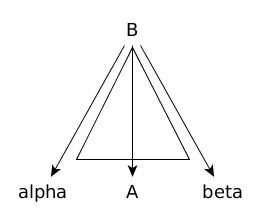
\includegraphics[scale=0.6]{Chapters/Img/c04_01.png}\\
\end{center} 
Quindi in pratica i follow(A) li trovo guardando le produzioni con A dopo la freccia. 
$\alpha $ e $\beta $ sono espressioni con lunghezza qualsiasi mentre A \'e un non treminale.\\[5pt]
Se tipo ho abCdEFGhi come lo spacco in $\alpha B\beta$? Vai in ordine, se vuoi calcolarti i follow di C allora C sarà la tua B.

\noindent\rule{16cm}{0.4pt}

\begin{center}
    \begin{tabular}{l}
        Calcolo follow(B), guardo produzioni $A \rightarrow \alpha B \beta$\\
        Metti $\$$ per tutti i non terminali\\
        Per le produzioni $A\rightarrow aB$ tutti i follow di A vanno in B\\
        Per $A\rightarrow aBb$ tutti i first(b) meno epsilon vanno in follow(B)\\
        Per $A\rightarrow aBb$ con epsilon appartenente ai first(b) allora aggiungi anche i follow(A) ai follow(B)\\
    \end{tabular}
\end{center}

\noindent\rule{16cm}{0.4pt}

%%%%%%%%%%%%%%%%%%%%%%%%%%%%%%%%%%%%%%%%%%%%%%%%%%%%%%%%%%%%%%%%%%%%%%%%%%%%%%%%%%%%%%%
\subsection{Esempio}

$S \rightarrow aABb$\\
$A \rightarrow Ac|d$\\
$B \rightarrow CD$\\
$C \rightarrow e|\varepsilon$\\
$D \rightarrow f|\varepsilon$\\

\begin{tabular}{ccc}
              &   First                     &   Follow      \\    
    $S=$      &    $\{ a \}$                &   $\{ \$ \}$        \\
    $A=$      &    $\{ d \}$                &   $\{e,f,b$ (da $S \rightarrow aABb$), c (da $A \rightarrow Ac$)$\}$ \\
    $B=$      &    $\{ e,f,\varepsilon \}$     &   $\{b \text{ (da } S \rightarrow aABb)\}$   \\
    $C=$      &    $\{ a,\varepsilon \}$       &   $\{f \text{ (da } B \rightarrow CD)\}$      \\
    $D=$      &    $\{ f,\varepsilon \}$       &   $\{\}$      \\
\end{tabular}\\[5pt]
Poi i follow(B) vanno in D perch\'e ho $B\rightarrow CD$ e anche in C perch\'e D pu\'o essere $\epsilon$.

%%%%%%%%%%%%%%%%%%%%%%%%%%%%%%%%%%%%%%%%%%%%%%%%%%%%%%%%%%%%%%%%%%%%%%%%%%%%%%%%%%%%%%%
\subsection{Esempio}

$S \rightarrow aA|bBc$\\
$A \rightarrow Bd|Cc$\\
$B \rightarrow e|\varepsilon$\\
$C \rightarrow f|\varepsilon$\\

\begin{tabular}{ccc}
              &   First                   &   Follow            \\    
    $S=$      &    $\{ a, b \}$           &   $\{ \$ \}$        \\
    $A=$      &    $\{ e,d,f,c \}$        &   $\{ \$,(?) \}$    \\
    $B=$      &    $\{ e,\varepsilon \}$     &   $\{ c,d \}$       \\
    $C=$      &    $\{ f,\varepsilon \}$     &   $\{ c \} $        \\
\end{tabular}
Occhio che nei first di A non ci va $ \varepsilon $ perch\'e 
ci può essere dalla sostituzione con B ma subito dopo hai d quindi in questo caso il first \'e d
%%%%%%%%%%%%%%%%%%%%%%%%%%%%%%%%%%%%%%%%%%%%%%%%%%%%%%%%%%%%%%%%%%%%%%%%%%%%%%%%%%%%%%%
\subsection{Esempio}

$E \rightarrow TE'$\\
$E' \rightarrow +TE'|\varepsilon$\\
$T \rightarrow FT'$\\
$T' \rightarrow *FT'|\varepsilon$\\
$F \rightarrow (E)|id $\\

\begin{tabular}{cccc}
              &   First                     &   Follow      &                               \\    
    $E=$      &    $\{ id, ( \}$            &   $\{\$,)\}$  &                               \\
    $E'=$     &    $\{ +, \varepsilon \}$      &   $\{\}$      &   ed eredita i follow di E    \\
    $T=$      &    $\{ id, ( \}$            &   $\{+\}$     &   ed eredita i follow di E,E' \\
    $T'=$     &    $\{ *, \varepsilon \}$      &   $\{\}$      &   ed eredita i follow di T    \\    
    $F=$      &    $\{ id, ( \}$            &   $\{*\}$     &   ed eredita i follow di T, T'\\
    & & Quindi diventa: & \\
    $E=$      &    $\{ id, ( \}$            &   $\{\$,)\}$      &   \\
    $E'=$     &    $\{ +, \varepsilon \}$      &   $\{\$,)\}$      &   \\
    $T=$      &    $\{ id, ( \}$            &   $\{+, \$ , ) \}$     &   \\
    $T'=$     &    $\{ +, \varepsilon \}$      &   $\{+, \$ , ) \}$     &   \\    
    $F=$      &    $\{ id, ( \}$            &   $\{*, +, \$ , ) \}$  &   \\
\end{tabular}\\[5pt]

Parsing di \lq\lq$id+id*id\$$\rq\rq\ $E \rightarrow TE' \rightarrow FT'E' \rightarrow idT'E' \rightarrow ...$ 

%%%%%%%%%%%%%%%%%%%%%%%%%%%%%%%%%%%%%%%%%%%%%%%%%%%%%%%%%%%%%%%%%%%%%%%%%%%%%%%%%%%%%%%%%%%%%%%%%%%%%%%%%%%%
\section{Tabella di parsing}
    Nella cella [A,b] metto le produzioni $A \rightarrow \beta \ / \ b \in first(\beta)$.
    Se epsilon appartiene ai first devi anche controllare che il terminale sia contenuto nei follow del non terminale\\[5pt]
\begin{tcolorbox}\begin{center}
    Quindi in [A, b] metto $(A \rightarrow \beta) \in P \ / \ b \in first(\beta)$ e se $\varepsilon \in first(\beta) \implies b \in follow(A) $. 
\end{center}\end{tcolorbox}

%%%%%%%%%%%%%%%%%%%%%%%%%%%%%%%%%%%%%%%%%%%%%%%%%%%%%%%%%%%%%%%%%%%%%%%%%%%%%%%%%%%%%%%%%%%%%%%%%%%%%%%%%%%%%%%%%%%%%%%%%%%%%%%%%%%%
\subsection{Algoritmo di costruzione della tabella di parsing predittivo top-down}

\begin{center}
    \begin{tabular}{ll}
        input   &   G=(V,T,S,P) \\
        output  &   Tabella T di parsing predittivo top-down se G \'e LL(1)\\
    \end{tabular}
\end{center}

\begin{lstlisting}
    foreach((A -> alpha) in P){
        forall b in first(alpha), poniamo A -> alpha in T[A, b];
        if(epsilon in first(alpha)){
            forall x in follow(A) poniamo A -> alpha in T[A, x];
        }
    }
    
    poniamo error() in tutte le entry di T che sono rimaste vuote;

    if(la tabella non ha entry multiply-defined)
        G e'' LL(1);

\end{lstlisting}

%%%%%%%%%%%%%%%%%%%%%%%%%%%%%%%%%%%%%%%%%%%%%%%%%%%%%%%%%%%%%%%%%%%%%%%%%%%%%%%%%%%%%%%
\subsection{Esempio}

$E \rightarrow E+T|T $\\
$T \rightarrow T*F|T $\\
$F \rightarrow (E)|id $\\

\begin{center}
    \begin{tabular}{|cccc|}
        \hline
                &   First                     &   Follow                               &                           \\    
        \hline
        $E=$      &    $\{ (, id \}$            &   $\{ \$, +, ) \}$                     &   $\{ \$, +, ) \}$        \\
        $T=$      &    $\{ (, id \}$            &   $\{ * \}$ ed eredita i follow di E   &   $\{ \$, +, *, ) \}$     \\
        $F=$      &    $\{ (, id \}$            &   $\{ \}$ ed eredita i follow di T     &   $\{ \$, +, *, ) \}$     \\
        \hline
    \end{tabular}
    \begin{tabular}{|l|l|}
        \hline
            &   id  \\
        \hline
        E   &   $E \rightarrow E + T $  \\
            &   $E \rightarrow T $      \\
        \hline
    \end{tabular}
    Guardo se \'e LL(1)\\
\end{center}

Pur non sviluppando tutta la tabella si vede che ci sono entry multiple \textbf{quindi non \'e LL(1)}.

%%%%%%%%%%%%%%%%%%%%%%%%%%%%%%%%%%%%%%%%%%%%%%%%%%%%%%%%%%%%%%%%%%%%%%%%%%%%%%%%%%%%%%%%%%%%%%%%
\section{Algoritmi di Parsing}
\begin{center}
    \begin{tabular}{ll}
        input buffer    &   w$\$$   \\
        stack           &   bottom [$ \$ \qquad $] top \\
        parsing table   &   con tante righe quante non terminali, tante colonne quante terminali ($ \$ $ incluso)\\
                        &   in ogni cella metto un'eventuale trasformazione o \lq\lq error \rq\rq \\
    \end{tabular}
\end{center}

%%%%%%%%%%%%%%%%%%%%%%%%%%%%%%%%%%%%%%%%%%%%%%%%%%%%%%%%%%%%%%%%%%%%%%%%%%%%%%%%%%%%%%%%%%%%%%%%
\subsection{Algoritmo di parsing non-ricorsivo}
\begin{center}
    \begin{tabular}{ll}
        input   &   stringa w, tabella parsing non ricorsivo T, per G\\
        output  &   derivazione leftmost di w se $w \in L(G)$, error() altrimenti\\
    \end{tabular}
\end{center}

\begin{lstlisting}
    //non terminali e gli stati del grafo sono la stessa cosa
    //init
    buffer = {w$}; //meglio $w^r
    stack.push($S); //stack di terminali e non terminali

    let b = buffer.pop() //il primo simbolo di w 
    let x = stack.top()  

    while(x != $){
        if(x == b){ //ho il carattere giusto e lo brucio
            stack.pop(x);
            b = buffer.nextChar();
        } else if(x e'' terminale){ 
            //sono arrivato ad un terminale diverso da quello della stringa
            error();
        } else if(T[x,b] contiene x -> Y1...Yn){ //x e' un non terminale (nello stack)
            //se la tabella di parsing contiene una entry 
            cout << x -> Y1...Yn;
            stack.pop(x);
            stack.push(Yn...Y1); //li pusha al contrario
                            //se ho una epsilon non la pusho
        }
        x = stack.top()
    }
\end{lstlisting}

%%%%%%%%%%%%%%%%%%%%%%%%%%%%%%%%%%%%%%%%%%%%%%%%%%%%%%%%%%%%%%%%%%%%%%%%%%%%%%%%%%%%%%%%%%%%%%%%%%%%%%%%%
\subsection{Esempio}
$E \rightarrow TE'$ \\
$E' \rightarrow +TE'|\varepsilon$\\
$T \rightarrow FT'$\\
$T' \rightarrow *FT'|\varepsilon$\\
$F \rightarrow id$\\
\begin{center}

    \textbf{First and Follow}\\
    \begin{tabular}{|c|c|c|}
        \hline
        \textbf{Non terminale} & \textbf{First} & \textbf{Follow} \\
        \hline
        E   &   id                  &   $\$$    \\
        \hline
        E'  &   +, $\varepsilon$    &   $\$$    \\
        \hline
        T   &   id                  &   +, $\$$    \\
        \hline
        T'  &   *, $\varepsilon$    &   +, $\$$    \\
        \hline
        F   &   id                  &   +, *, $\$$    \\
        \hline
    \end{tabular}\\[5pt]

    \textbf{Tabella di parsing}\\
    \begin{tabular}{|c|c|c|c|c|}
        \hline
                &   id                      &   +                           &   *   &   $\$$    \\
        \hline
            E   &   $E \rightarrow TE'$     &                               &     &      \\
        \hline
            E'  &                           &   $E' \rightarrow +TE'$        &     &   $E' \rightarrow \varepsilon $    \\
        \hline
            T   &   $T \rightarrow FT'$     &                               &      &      \\
        \hline
            T'  &                           &   $T' \rightarrow \varepsilon$    &   $T' \rightarrow *FT'$   &   $T' \rightarrow \varepsilon$    \\
        \hline
            F   &   $F \rightarrow id$      &                               &      &       \\
        \hline
    \end{tabular}\\[5pt]
    \textbf{Passi dell'algoritmo}\\
    \begin{tabular}{|l|l|l|}
        \hline
        pila & input & output \\
        \hline
        $\$ $ \underline{E}  &   \underline{$id$}$+id*id\ \$ $  &   $E \rightarrow TE'$ \\
        \hline
        $\$ $ E \underline{T'}  &   &   $T \rightarrow FT' $ \\
        \hline
        $\$ $ E T' \underline{F}  &   &   $F \rightarrow id $ \\
        \hline
        $\$ $ E T' \underline{id}  &    &   \\
        \hline
        $\$ $ E' \underline{T'}  &  \underline{$+$}$ id *id\ \$$  &   $T' \rightarrow \varepsilon $ \\
        \hline
        $\$ $ \underline{E'}  &    &   $E' \rightarrow TE'$ \\
        \hline
        $\$ $ E' T \underline{+}  &   \underline{$id$}$*id\ \$ $  &   \\
        \hline
        $\$ $ E' \underline{T}  &     &   \\
        \hline
            &     ...Avanti cos\i     &   \\
        \hline
    \end{tabular}
\end{center}
\Tree[.E [.T [.F id ] [.T' $\varepsilon$ ] ] [.E' + [.T  [.F id ] [.T' * [.F id ] [.T' $\varepsilon$ ] ] ] [.E' $\varepsilon$ ] ] ]

%%%%%%%%%%%%%%%%%%%%%%%%%%%%%%%%%%%%%%%%%%%%%%%%%%%%%%%%%%%%%%%%%%%%%%%%%%%%%%%%%%%%%%%%%%%%%%%%
\subsection{Esercizio}
$S \rightarrow aA | bB$\\
$A \rightarrow c $\\
$B \rightarrow d $\\

$w = ac\$ $ \\

Parsing: $S \implies aA \implies ac $\\

\begin{center}
    \textbf{First and Follow}\\[5pt]
    \begin{tabular}{|c|c|c|}
        \hline
        \textbf{Non terminali} & \textbf{First} &   \textbf{Follow}\\
        \hline
        S   &   a, b    &   $\$$ \\
        \hline
        A   &   c    &   $\$$ \\
        \hline
        B   &   d    &   $\$$ \\
        \hline
    \end{tabular}\\[10pt]
    \textbf{Tabella di parsing con le produzioni di G}\\[5pt]
    \begin{tabular}{|l|l|l|l|l|l|}
        \hline
            &   a   &   b   &   c   &   d   &   $\$$    \\
        \hline
        S   &   $S \rightarrow aA$   &    $S \rightarrow bB$   &      &      &      \\
        \hline
        A   &      &      &  $A \rightarrow c$     &      &      \\
        \hline
        B   &      &      &       &  $B \rightarrow d$    &      \\  
        \hline
    \end{tabular}
\end{center}

%%%%%%%%%%%%%%%%%%%%%%%%%%%%%%%%%%%%%%%%%%%%%%%%%%%%%%%%%%%%%%%%%%%%%%%%%%%%%%%%%%%%%%%%%%%%%%%%%%%%%%%%%%%%%%%%%%%%%%%%%%%%%%%%
\section{Grammatica Ricorsiva Sinistra}
Una grammatica G esibisce \textbf{left recursion} se $\exists\ A \in (V\backslash T) \ / \ A \rightarrow^* A \alpha ,\ \alpha \in V^*$

La left recursion \'e immediata se G ha almeno una produzione del tipo $A \rightarrow A \alpha$ (ovvero se succede nel passato).
Nell'esempio di prima c'era left recursion immediata nei primi due casi ($E \rightarrow E\alpha \land T \rightarrow T\alpha $).

\begin{tcolorbox}\begin{center}
    Proposizione: ogni grammatica che esibisce left recursion \textbf{non \'e LL(1)}.
\end{center}\end{tcolorbox}

\begin{tcolorbox}\begin{center}
    Proposizione: ogni grammatica che nella tabella di parsing ha pi\'u di una entry in una cella \textbf{non \'e LL(1). Altrimenti lo \'e}.
\end{center}\end{tcolorbox}

\begin{tcolorbox}\begin{center}
    Se una grammatica \'e LL(1) $\implies$ non da conflitti nella tabella di parsing $\implies$ \'e una grammatica libera.
\end{center}\end{tcolorbox}

$A \rightarrow B$\\
$B \rightarrow Aa$\\
Esempio di left recursion in pi\'u passi.

%%%%%%%%%%%%%%%%%%%%%%%%%%%%%%%%%%%%%%%%%%%%%%%%%%%%%%%%%%%%%%%%%%%%%%%%%%%%%%%%%%%%%%%%%%%%%%%%%%
\section{Eliminazione Left Recursion immediata}

%%%%%%%%%%%%%%%%%%%%%%%%%%%%%%%%%%%%%%%%%%%%%%%%%%%%%%%%%%%%%%%%%%%%%%%%%%%%%%%%%%%%%%%%%%%%%%%%%%
\subsection{Esempio}
$A \rightarrow A \alpha | \beta $, con $\beta \not= A \land \alpha \not= \varepsilon$ diventa:\\
$A \rightarrow \beta A'$\\
$A' \rightarrow \alpha A' | \varepsilon$\\

Pi\'u in generale
$A \rightarrow A\alpha _1 | ... | A\alpha _n | \beta _1 | ... | \beta _n, \quad \beta _1, ..., \beta _n \not= A_y,\quad \alpha_1,...,\alpha_n \not= \varepsilon$ diventa\\
$A \rightarrow \beta _1 A'|...|\beta _n A' $\\
$A' \rightarrow \alpha _1 A'|...|\alpha _n A' | \varepsilon $\\
Ho introdotto A' nuovo non terminale in G.

%%%%%%%%%%%%%%%%%%%%%%%%%%%%%%%%%%%%%%%%%%%%%%%%%%%%%%%%%%%%%%%%%%%%%%%%%%%%%%%%%%%%%%%%%%%%%%%%%%
\subsection{Esempio}

\noindent\fbox{
    \begin{minipage}[t]{0.48\linewidth}
        Eliminare Left Recursion immediata da:\\
        $E \rightarrow E + T | T $\\
        $T \rightarrow T*F|F  $\\
        $F \rightarrow (E)|id $\\
    \end{minipage}
}
\hfill
\fbox{
    \begin{minipage}[t]{0.48\linewidth}
        Diventa:\\
        $E \rightarrow TE' $\\
        $E' \rightarrow +TE'|\varepsilon $\\
        $T \rightarrow FT'  $\\
        $T' \rightarrow *FT' | \varepsilon $\\
        $F \rightarrow (E)|id $\\
    \end{minipage}
}

\begin{tabular}{ccc}
              &   First                    &   Follow                   \\    
    $E=$      &    $\{ id, ( \}$           &   $\{ \$, ) \}$            \\
    $E'=$     &    $\{ +, \varepsilon \}$     &   $\{ \$, ) \}$            \\
    $T=$      &    $\{ id, ( \}$           &   $\{ +, \$, ) \}$         \\
    $T'=$     &    $\{ *, \varepsilon \}$     &   $\{ +, \$, ) \}$         \\
    $F=$      &    $\{ id, ( \}$           &   $\{ *, +, \$, ) \}$      \\
\end{tabular}

%%%%%%%%%%%%%%%%%%%%%%%%%%%%%%%%%%%%%%%%%%%%%%%%%%%%%%%%%%%%%%%%%%%%%%%%%%%%%%%%%%%%%%%%%%%%%%%%%%%%%%%%%%%%%%%%%%%%%%%%%%%%%%%%%%%%
\subsubsection{Tabella di parsing}

\begin{tabular}{|c|c|c|c|c|c|c|}
    \hline
        &   id      &    +   &   *   &   (   &   )   &   $\$$\   \\
    \hline
    E   &   $E \rightarrow TE' $    &  & &   $E \rightarrow TE' $   &      &   $\$$\   \\
    \hline
    E'  &   &    $E' \rightarrow +TE' $ &      &      &   $E' \rightarrow \varepsilon $   &  $E' \rightarrow \varepsilon $   \\
    \hline
    T   &   $T \rightarrow FT' $    &  & &   $T \rightarrow FT' $   & &   $\$$\   \\
    \hline
    T'  &   & $T' \rightarrow \varepsilon $ & $T' \rightarrow *FT' $   & &   $T' \rightarrow \varepsilon $   &   $T' \rightarrow \varepsilon $ \\
    \hline
    F   &   $F \rightarrow id $ &  &  &   $F \rightarrow (E) $   &   )   &   $\$$\   \\
    \hline
\end{tabular}\\[5pt]
I campi vuoti sono error, non ci sono multiple entries quindi \'e LL(1).

%%%%%%%%%%%%%%%%%%%%%%%%%%%%%%%%%%%%%%%%%%%%%%%%%%%%%%%%%%%%%%%%%%%%%%%%%%%%%%%%%%%%%%%%%%%%%%%%%%
\subsection{Esempio}

Eliminare Left Recursion immediata da:\\
$E \rightarrow E + E | E * E | (E) |id $\\

Diventa:\\
$E \rightarrow (E)E' | id E' $\\
$E' \rightarrow +EE'| *EE' | \varepsilon $\\

(Parte della tabella tanto non serve tutta)
\begin{tabular}{|cccc|}
    \hline
              &   First                    &   Follow                                   &                       \\    
    \hline
    $E=$      &    $\{ id, ( \}$           &   $\{ \$, ), +, * \}$ ed i follow di E'    & $\{ \$, ), +, * \}$   \\
    $E'=$     &    $\{ +, *, \varepsilon \}$         &   $\{ \}$ ed i follow di E                 & $\{ \$, ), +, * \}$   \\
    \hline
\end{tabular}

Visto che ho almeno una entry multipla la grammatica non \'e LL(1).

L'eliminazione della left recursion ci ha dato un grammatica che non \'e comunque LL(1). Nel nostro caso \'e anche ambigua.

\begin{tcolorbox}\begin{center}
    Lemma: L'eliminazione della left recursion NON elimina \textbf{l'ambiguit\'a}.
\end{center}\end{tcolorbox}

%%%%%%%%%%%%%%%%%%%%%%%%%%%%%%%%%%%%%%%%%%%%%%%%%%%%%%%%%%%%%%%%%%%%%%%%%%%%%%%%%%%%%%%%%%%%%%%%%%
\section{Left Factoring}

$S \rightarrow aSb | ab$

\begin{tabular}{|c|c|c|c|}
    \hline
        &   a                   &   b   &   $\$$    \\
    \hline
    S   &   $S \rightarrow aSb$ &       &           \\
        &   $S \rightarrow ab$  &       &           \\
    \hline
\end{tabular}
La grammatica non \'e LL(1).\\

Possiamo per\'o fattorizzare le produzioni considerando una parte che \'e a sinistra ed \'e comune a pi\'u 
produzioni, per ottenere una \textbf{grammatica LL(1)} che genera lo stesso linguaggio.

$S \rightarrow aA'$\\
$A' \rightarrow Sb|b$\\

%%%%%%%%%%%%%%%%%%%%%%%%%%%%%%%%%%%%%%%%%%%%%%%%%%%%%%%%%%%%%%%%%%%%%%%%%%%%%%%%%%%%%%%%%%%%%%%%%%%%%%%%%%%%%%%%%%%%%%%%%%%%%%%%%%%%
\subsubsection{DEF}
Una grammatica G pu\'o essere fattorizzata a sinistra quando esistono almeno due produzioni $A \rightarrow \alpha\beta _1$ e
$A \rightarrow \alpha\beta _2$ per qualche $A \in V\backslash T,\ \alpha ,\beta _1, \beta _2 \in V^* \land \alpha $ non comincia per $A$.

%%%%%%%%%%%%%%%%%%%%%%%%%%%%%%%%%%%%%%%%%%%%%%%%%%%%%%%%%%%%%%%%%%%%%%%%%%%%%%%%%%%%%%%%%%%%%%%%%%%%%%%%%%%%%%%%%%%%%%%%%%%%%%%%%%%%
\subsubsection{DEF}
G pu\'o essere fattorizzata a sinistra se:
$A \rightarrow \alpha \beta _1,\ A \rightarrow \alpha\beta _2 \in P$ con \\
$\alpha , \beta _1, \beta _2 \in V^*, \alpha $ non ha $A$ come primo simbolo, $A \in V\backslash T$

%%%%%%%%%%%%%%%%%%%%%%%%%%%%%%%%%%%%%%%%%%%%%%%%%%%%%%%%%%%%%%%%%%%%%%%%%%%%%%%%%%%%%%%%%%%%%%%%%%%%%%%%%%%%%%%%%%%%%%%%%%%%%%%%%%%%
\subsubsection{Lemma}
Se G pu\'o essere fattorizzata a sinistra allora \textbf{G non \'e LL(1)}.

%%%%%%%%%%%%%%%%%%%%%%%%%%%%%%%%%%%%%%%%%%%%%%%%%%%%%%%%%%%%%%%%%%%%%%%%%%%%%%%%%%%%%%%%%%%%%%%%%%
\section{Algoritmo di fattorizzazione a sinistra}
\begin{lstlisting}
    foreach(A in V\T){
        trovare il prefisso piu lungo comune a due o piu produzioni per A, chiamato alpha 
        if(alpha != epsilon){
            sostituire A -> alpha beta_1|...|alpha beta_n|Y_1|...|Y_k
            con A -> alpha A' | Y_1 | Y_k 
            con A' -> beta_1 | ... | beta_n e A' nuovo simbolo
        }
    }
\end{lstlisting}

manca roba

%%%%%%%%%%%%%%%%%%%%%%%%%%%%%%%%%%%%%%%%%%%%%%%%%%%%%%%%%%%%%%%%%%%%%%%%%%%%%%%%%%%%%%%%%%%%%%%%%%
\chapter{Parsing Bottom Up}
%Zampedri
\begin{center}
    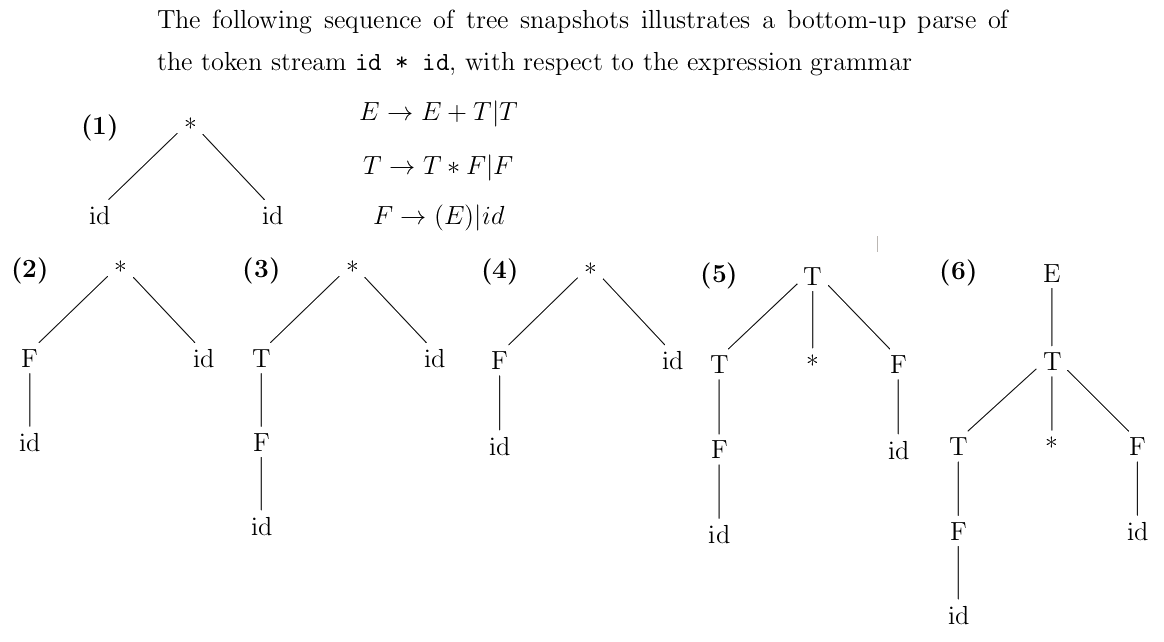
\includegraphics[scale=0.4]{Chapters/Img/c04_02.png}\\
\end{center}

\begin{tabular}{ll}
    Riduzione:      &   $id * id,\ F * id,\ T * id,\ T * F,\ T,\ E$\\
    Derivazione:    &   $E \rightarrow T \rightarrow T * F \rightarrow T * id \rightarrow F * id \rightarrow id * id$\\
\end{tabular}

%%%%%%%%%%%%%%%%%%%%%%%%%%%%%%%%%%%%%%%%%%%%%%%%%%%%%%%%%%%%%%%%%%%%%%%%%%%%%%%%%%%%%%%%%%%%%%%%%%%%%%%%%%%%%%%%%%%%%%%%%%%%%%%%%%%%
\section{Reductions}
La \textbf{riduzione} \'e l'operazione inversa della \textbf{derivazione}.
Posso pensare al parsing bottom up come al processo di riduzione di una stringa w allo start symbol della grammatica.
In ogni step di riduzione una sottostringa che matcha con il body di una produzione viene ridotta con la testa della produzione.

Le scelte critiche sono quando ridurre e cosa ridurre.

%%%%%%%%%%%%%%%%%%%%%%%%%%%%%%%%%%%%%%%%%%%%%%%%%%%%%%%%%%%%%%%%%%%%%%%%%%%%%%%%%%%%%%%%%%%%%%%%%%%%%%%%%%%%%%%%%%%%%%%%%%%%%%%%%%%%
\section{Handle Pruning}
Chiamo handle una sottostringa che matcha con il body di una produzione, e la sua riduzione \'e un passo inverso, al contrario, di una 
rightmost derivation.

\begin{center}
    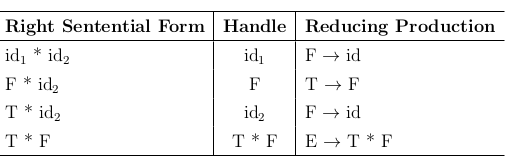
\includegraphics[scale=0.6]{Chapters/Img/c04_03.png}\\
\end{center}

%%%%%%%%%%%%%%%%%%%%%%%%%%%%%%%%%%%%%%%%%%%%%%%%%%%%%%%%%%%%%%%%%%%%%%%%%%%%%%%%%%%%%%%%%%%%%%%%%%%%%%%%%%%%%%%%%%%%%%%%%%%%%%%%%%%%
\section{Shift reduce parsing}
\'E una forma di bottom up parsing in cui mi appoggio ad uno stack contenente i simboli della grammatica e un buffer per la input string
da parsare. 

\begin{lstlisting}
    //init
    stack = $;
    buffer = w$;
    //faccio uno scan da sx a dx e shifto simboli dal buffer allo stack 
    //quando nello stack posso fare una riduzione sostituisco
    //vado avanti fince' non ho un error o finisce il buffer
\end{lstlisting}
Sembra che qualsiasi stringa possa essere parsata, basta continuare a shiftare???

\begin{center}
    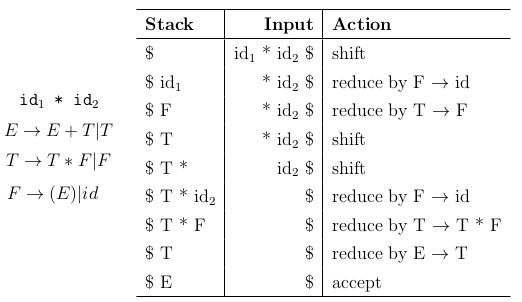
\includegraphics[scale=0.6]{Chapters/Img/c04_04.png}\\
\end{center}

Ho \textbf{shift} quando passo un simbolo dal buffer allo stack, \textbf{reduce} quando applico una riduzione sul top dello stack 
(mai inside), \textbf{accept} se sono in fondo al buffer e ho quindi parsato correttamente la stringa, \textbf{error} nol va!

L'algoritmo shift reduce non funziona per tutte le grammatiche, pu\'o essere che in certi casi mi trovi in situazioni dove non 
so decidere se fare shift o reduce o non so quale reduce scegliere (reduce conflicts).

%%%%%%%%%%%%%%%%%%%%%%%%%%%%%%%%%%%%%%%%%%%%%%%%%%%%%%%%%%%%%%%%%%%%%%%%%%%%%%%%%%%%%%%%%%%%%%%%%%%%%%%%%%%%%%%%%%%%%%%%%%%%%%%%%%%%
\subsection{Esempio}

\begin{center}
    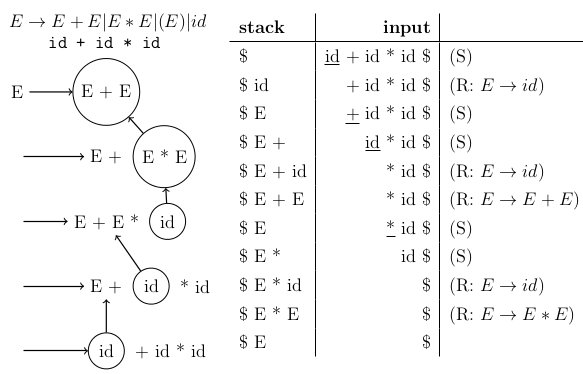
\includegraphics[scale=0.6]{Chapters/Img/c04_05.png}\\
\end{center}

%%%%%%%%%%%%%%%%%%%%%%%%%%%%%%%%%%%%%%%%%%%%%%%%%%%%%%%%%%%%%%%%%%%%%%%%%%%%%%%%%%%%%%%%%%%%%%%%%%%%%%%%%%%%%%%%%%%%%%%%%%%%%%%%%%%%
\section{LR parsing}
Il metodo pi\'u usato \'e LR(k) parsing con 
\begin{tabular}{ll}
    L   &   left to right input scan\\
    R   &   rightmost derivation costruita inversamente\\
    (k) &   numero di input symbol lookahead messi per prendere le decisioni\\
\end{tabular}

Se ometto k assumo che sia k = 1 (LR = LR(1)). Una grammatica \'e LR(1) se capace di parsare in shift reduce le stringhe (riconosce gli 
handles sul top dello stack).

%%%%%%%%%%%%%%%%%%%%%%%%%%%%%%%%%%%%%%%%%%%%%%%%%%%%%%%%%%%%%%%%%%%%%%%%%%%%%%%%%%%%%%%%%%%%%%%%%%%%%%%%%%%%%%%%%%%%%%%%%%%%%%%%%%%%
\subsection{LR(0) Automaton}
Per prendere decisioni critiche mi serve tener traccia dello stato in cui mi trovo nel parsing. Per rappresentare gli stati uso gli items;
un item \'e una produzione con un punto: $A \rightarrow XYZ$ codifica 4 items: 
$A \rightarrow .XYZ,\ A \rightarrow X.YZ,\ A \rightarrow XY.Z,\ A \rightarrow XYZ.$.
La produzione $A \rightarrow \varepsilon$, mi produce solo un item $A \rightarrow\ .\ $. \\


Intuitivamente $A \rightarrow X.YZ$ mi dice che ho gi\'a visto X ma non YZ.

\textbf{canonical LR(0) collection} \'e un set di item LR(0) che mi permettono di costruire DFA in grado di prendere decisioni
precise per il parsing; in particolare ogni stato nel automa rappresenta un set di item del canonical LR(0) collection.

Per costruire l'automa definisco una grammatica aumentata e le funzioni CLOSURE e GOTO. 
Data G con start symbol S, G' \'e una grammatica aumentata di G ed ha la produzione $S' \rightarrow S$ (start symbol S').
Questo serve essenzialmente per poter annunciare la fine del parsing.

\subsubsection{Closure of Item Sets}
Dato I set di item per G, CLOSURE(I) \'e il set degli item costruito da I $ / $ \\[5pt]
\begin{tabular}{ll}
    i)  &   inizialmente closure(I) = I \\
    ii) &   se $(A \rightarrow \alpha . B \beta) \in closure(I) \land (B \rightarrow \gamma) \in P$ 
           aggiungi $B \rightarrow .\gamma$ a closure(I) (se non gi\'a presente).\\
\end{tabular}\\[5pt]

Vado avanti ricorsivamente finch\'e non ho aggiunto tutto quello che potevo.

\begin{center}
    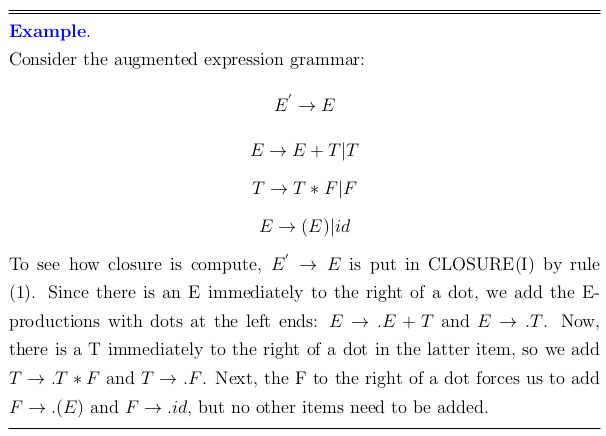
\includegraphics[scale=0.6]{Chapters/Img/c04_06.png}\\
\end{center}

Sembra che $E' \rightarrow E$ sia lo stesso di $E' \rightarrow .E$; in pratica per ogni item guardo se ho un non terminale subito a 
destra del punto e casomai inserisco tutti gli item con tale simbolo in testa.

\begin{lstlisting}
    J = I;
    repeat{
        foreach( [A -> alpha . B beta] in J) 
            foreach( [B -> gamma] in G)
                if( [B -> .gamma] not in J)
                    J.add( [B -> .gamma] );
    } until (saturation) //nothing more can be added!
\end{lstlisting}

%%%%%%%%%%%%%%%%%%%%%%%%%%%%%%%%%%%%%%%%%%%%%%%%%%%%%%%%%%%%%%%%%%%%%%%%%%%%%%%%%%%%%%%%%%%%%%%%%%%%%%%%%%%%%%%%%%%%%%%%%%%%%%%%%%%%
\subsubsection{GOTO funtion}
GOTO(I, X), I set of items, $X \in V$, $\triangleq closure( \{[A \rightarrow \alpha X. \beta] \ / \ [A \rightarrow \alpha .X \beta] \in I \} ) $. 

In pratica lo uso per definire le transizioni nell'automa LR(0); gli stati sono set di item e le transizioni sono definite dai GOTO(I, X) 
(dallo stato I per il simbolo X).

%%%%%%%%%%%%%%%%%%%%%%%%%%%%%%%%%%%%%%%%%%%%%%%%%%%%%%%%%%%%%%%%%%%%%%%%%%%%%%%%%%%%%%%%%%%%%%%%%%%%%%%%%%%%%%%%%%%%%%%%%%%%%%%%%%%%
\subsection{Esempio}

$ I = \{ [E' \rightarrow E.],\ [E \rightarrow E. +T] \}$
\begin{tabular}{|ll}
        &   $E' \rightarrow E$\\
   G =  &    $E \rightarrow E + T| T$\\
        &   $T \rightarrow T * F | F$\\
        &   $E \rightarrow (E)|id$\\
\end{tabular}\\[10pt]


$GOTO(I, +) = $
\begin{tabular}{|ll|}
    $[E \rightarrow E + .T]$,   &   Mi arriva +, scarto $[E' \rightarrow E.]$, tengo l'altro'    \\
    $[T \rightarrow .T * F]$,   &   Includo i primi item per le produzioni con T in testa    \\
    $[T \rightarrow .F]$,       &       \\
    $[F \rightarrow .(E)]$,     &   Visto che ho $[T \rightarrow .F]$ includo gli item con F\\
    $[F \rightarrow .id]$,      &       \\
\end{tabular}\\[10pt]

%%%%%%%%%%%%%%%%%%%%%%%%%%%%%%%%%%%%%%%%%%%%%%%%%%%%%%%%%%%%%%%%%%%%%%%%%%%%%%%%%%%%%%%%%%%%%%%%%%%%%%%%%%%%%%%%%%%%%%%%%%%%%%%%%%%%
\section{Algoritmo generazione canonical collection C}

Per trovare C, canonical collection of sets of LR(0) items for an augmented grammar G'.

\begin{lstlisting}
    C = [CLOSURE{S' -> S}]
    repeat{
        foreach(I in C){ //set of item I 
            foreach(X in V'){
                if(GOTO(I,X) != empty && not in C yet){
                    C.add(GOTO(I,X));
                }
            }
        }
    } until (saturation)
\end{lstlisting}

\section{Simple LR (SLR)}
SLR parsing consiste nella costruzione della grammatica dell'automa LR(0). Gli stati dell'automa sono set di item derivanti 
da C (canonical LR(0) collection) e le transizioni derivano dalla GOTO functions.

Lo start state dell'automa LR(0) \'e $CLOSURE({[S' \rightarrow .S]})$ (S' start symbol di G' grammatica aumentata).

Per prendere decisioni, immaginando di arrivare con la stringa $\gamma$ dallo stato 0 allo stato j; a questo punto posso shiftare il 
prossimo carattere a se j ha transizioni per a oppure ridurre. Gli item in j mi dicono cosa fare.

%%%%%%%%%%%%%%%%%%%%%%%%%%%%%%%%%%%%%%%%%%%%%%%%%%%%%%%%%%%%%%%%%%%%%%%%%%%%%%%%%%%%%%%%%%%%%%%%%%%%%%%%%%%%%%%%%%%%%%%%%%%%%%%%%%%%
\subsection{Esempio}

G = 
\begin{tabular}{|l}
    $E \rightarrow E + T|T$\\
    $T \rightarrow T * F | T$\\
    $F \rightarrow (E) | id $\\
\end{tabular}\\[10pt]

Aumento la grammatica con $E' \rightarrow E$.\\

Computo $CLOSURE( \{ E' \rightarrow E \} ):$ 
\begin{tabular}{|ll|}
    \hline
                    &   $ E' \rightarrow .E,$\\
                    &   $ E \rightarrow .E + T, $\\
                    &   $ E \rightarrow .T, $\\
    $I_0$ =         &   $ T \rightarrow .T * F, $\\
                    &   $ T \rightarrow .F, $\\
                    &   $ F \rightarrow .(E), $\\
                    &   $ F \rightarrow .id  $\\
    \hline
\end{tabular}\\[10pt]

Computo i sets 
\begin{tabular}{ll}
    $I_1$ =     &   $GOTO(I_0,E) = \{ E' \rightarrow E. ,\quad E \rightarrow E. + T \} $\\
    $I_2$ =     &   $GOTO(I_1, +) = \{ E \rightarrow E + .T,\quad T \rightarrow .T * F,\quad T \rightarrow .F,\quad F \rightarrow .(E),\quad F \rightarrow .id \} $\\
\end{tabular}
Quindi l'automa inizia con una forma di questo genere:
\begin{center}
    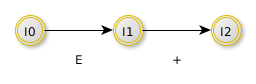
\includegraphics[scale=0.6]{Chapters/Img/c04_07.png}\\
\end{center}

%%%%%%%%%%%%%%%%%%%%%%%%%%%%%%%%%%%%%%%%%%%%%%%%%%%%%%%%%%%%%%%%%%%%%%%%%%%%%%%%%%%%%%%%%%%%%%%%%%%%%%%%%%%%%%%%%%%%%%%%%%%%%%%%%%%%
\section{The LR-Parsing Algorithm}
\begin{center}
    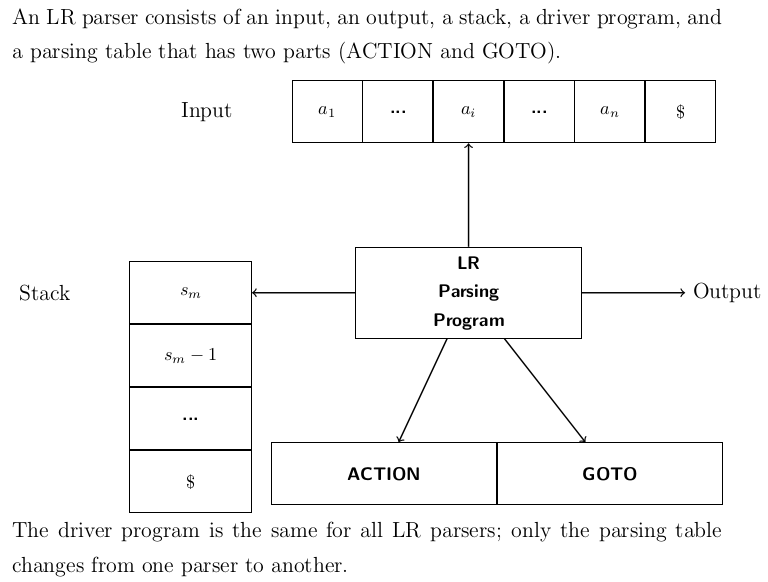
\includegraphics[scale=0.6]{Chapters/Img/c04_08.png}\\
\end{center}

\begin{tcolorbox}\begin{center}
    La differenza fra ACTION e GOTO \'e che le action sono applicate per input di terminali, GOTO per input di non terminali!
\end{center}\end{tcolorbox}

\subsection{Structure of LR Parsing Table}
La parsing table \'e strutturata in due parti: a parsing-action function \textbf{ACTION} and a goto funtion \textbf{GOTO}.
$ACTION[i,a], i \in States, a \in T \cup \{\$\}$ pu\'o assumere varie forme:

\begin{itemize}
    \item \textbf{Shift} $j,\ j \in States$ (shifta un carattere a ma usa j per rappresentarlo);\\
    \item \textbf{Reduce} $A \rightarrow \beta$ (riduce $\beta$ ad A)\\
    \item \textbf{Accept} \\
    \item \textbf{Error}\\
\end{itemize}

La prossima mossa del parser sar\'a leggere il simbolo corrente $a_i$ e lo stato in cima allo stack $s_m$. 
Guardo $ACTION[s_m,\ a_i]$ nella parsing action table. 

\subsection{LR Parsing Algorithm}

\begin{center}\begin{tabular}{ll}
    \textbf{Input}  &   string w, LR-parsing table con ACTION e GOTO per la grammatica G\\ 
    \textbf{Output} &   gli step di riduzione bottom-up per w o un errore\\
\end{tabular}\end{center}

\begin{lstlisting}
    stack.push(0);   //start state 0
    buffer.push(w$);
    * ip = leftChar(w); //pointer sul buffer
    repeat{
        n = stack.top();
        a = simbolo puntato da ip;
        if(T[n,a] == s_m){  //shift m
            push(a)
            push(m)
            move ip right
        } else if(T[n, a] = r_k con (k): A -> beta){    //reduce k
            pop 2^{|beta|} simboli;
            n' = stack.top(); 
            push(A);
            push m / T[A, n'] = g_m;
            cout << "A -> beta";
        } else if (T[n, a] == accept){
            accept();
        } else {
            error();
        }
    } until (accept() || error());
\end{lstlisting}

\subsection{Costruire SLR-Parsing Table}

Il metodo SLR inizia con items LR(0) ed un automa LR(0). Poi aumento la grammatica G, mi trovo C, GOTO e ACTION.\\[10pt]

\begin{tcolorbox}\begin{center}
    \textbf{G' non \'e SLR} se costruendo la parsing table ho dei \textbf{conflitti}. 
\end{center}\end{tcolorbox}

\begin{center}\begin{tabular}{ll}
    \textbf{Input}  &   G' grammatica arricchita\\ 
    \textbf{Output} &   Parsing table o un errore\\
\end{tabular}\end{center}

\begin{lstlisting}
    Define [I_0, ..., I_n] set items LR(0) per G'
    Define lo stato i nella tabella (ie row i) dopo l'elemento I_i come segue:

    * if (A -> alpha . a beta in I_i && GOTO(I_i, a) == I_j){
        T[i, a] = s_j;  // shift corrisponde ad un cambio di stato
    }
    * if (A -> alpha . in I_i){
        foreach(x in FOLLOW(A)){
            T[i,X] = r"A -> alpha"; // reduce
        }
    }
    * if (S' -> S. in I_i){ //ACCEPT
        T[i, $] = accept;
    }

    if(le azioni precedenti generano conflitti){
        throw Exception("G is not SLR");    //G non e' SLR
    } else {
        if(GOTO(I_i, A) == I_j){
            T[i, a] = g_j;  // goto
        }
        Put error() nelle entry vuote   //ERROR
        I_0 = CLOSURE(S' -> .S)
    }
\end{lstlisting}

\subsection{Esempio}
$1) E \rightarrow R + T$ \\
$2) E \rightarrow T$ \\
$3) T \rightarrow T * F$ \\
$4) T \rightarrow F$ \\
$5) F \rightarrow (E)$ \\
$6) F \rightarrow id$ \\

Arricchisco la grammatica con $E' \rightarrow E$, trovo \textbf{l'automa LR(0)}:

\begin{center}
    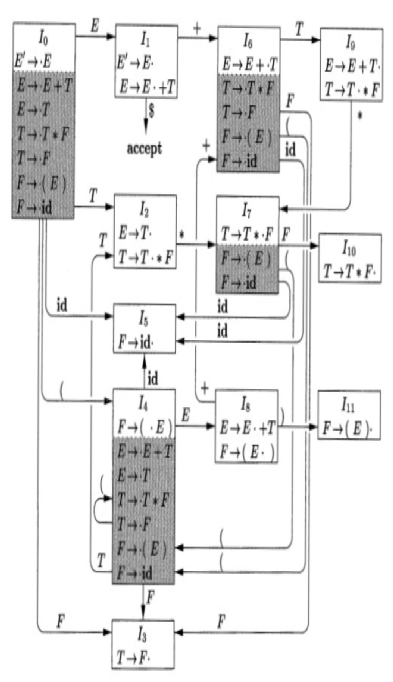
\includegraphics[scale=0.6]{Chapters/Img/c04_09.png}\\

    \begin{tabular}{l}
        \textbf{Osservazioni}\\
        Per ogni stato guardo solo i simboli dopo il punto negli item\\
        quindi ie l'item $F \rightarrow .(E)$ mi genera ACTION[0,(] = shift 4\\
        Da notare che da $I_1$ con $\$$ vado in ACCEPT perch\'e ho l'item $E' \rightarrow E.$\\
        La closure di $T \rightarrow T.*F = \emptyset$, \textbf{non espando i terminali}\\
        Considero $I_2$, dato l'item $E \rightarrow T.$ e dato che $FOLLOW(E) = \{ \$, +, ) \}$ \\
        $\implies ACTION[2,\$] = ACTION[2,+] = ACTION[2,)] = REDUCE E \rightarrow T$\\
    \end{tabular}\\[10pt]

    \textbf{In pratica l'automa mi crea la parsing table}

    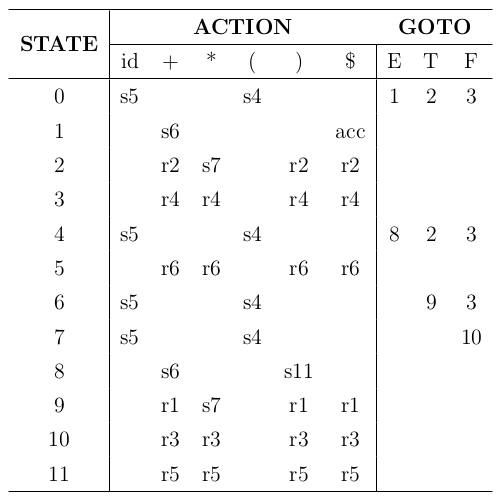
\includegraphics[scale=0.6]{Chapters/Img/c04_10.png}\\

    ie. $w= id * id + id$\\
    
    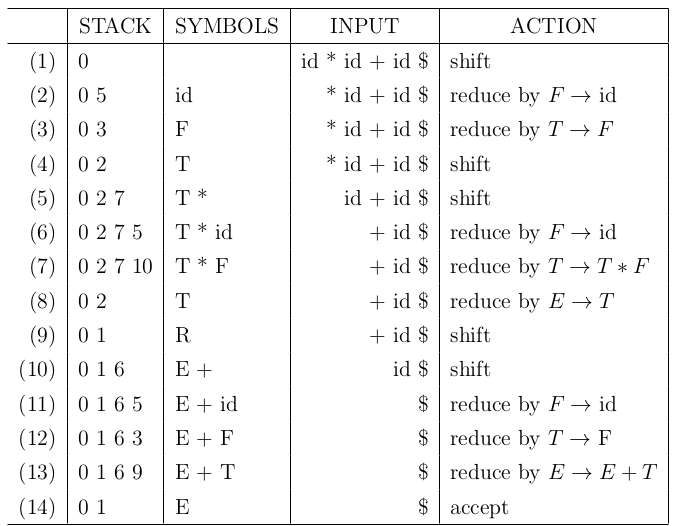
\includegraphics[scale=0.6]{Chapters/Img/c04_11.png}\\

    Sono in 0, mi arriva id faccio shift 5, pusho 5 sullo stack e id nei simboli; mi arriva *, faccio reduce $F \rightarrow id$, sostituisco 
    F a id nei simboli, faccio una pop dallo stack e mi trovo nello stato 0 con simbolo F che \'e una goto 3 (pusho 3). 
    Occhio che in (7) sono nello stato 10 e mi arriva +, faccio la reduce $T \rightarrow T * F$ e devo fare $|T * F| = 3$ pop dello stack.
\end{center}

\subsection{Shift/Reduce Conflicts}
SLR \'e una grammatica non ambigua, notare che ci sono grammatiche non ambigue che non sono SLR(1).
Considero G: 

$S \rightarrow L = R|R$\\
$L \rightarrow *R|id$\\
$R \rightarrow L$\\

La Canonical collection C \'e:\\
$I_0 = \{ S' \rightarrow .S,\ S \rightarrow .L = R,\ S \rightarrow .R,\ L \rightarrow .*R,\ L \rightarrow .id,\ R \rightarrow .L \}$\\
$I_1 = \{ S' \rightarrow S. \}$ (da $I_0$ mi arriva S)\\
$I_2 = \{ S  \rightarrow L.=R,\ R  \rightarrow L. \} $ (da $I_0$ mi arriva L)\\
$I_3 = \{ S  \rightarrow  R. \} $ (da $I_0$ mi arriva R)\\
$I_4 = \{ L \rightarrow *.R,\ R \rightarrow .L,\ L \rightarrow .*R,\ L \rightarrow .id \} $ (da $I_0$ mi arriva *, poi espando con le closure a cascata)\\
$I_5 = \{ L \rightarrow id.\}$ (da $I_0$ mi arriva id)\\
$I_6 = \{ S \rightarrow L = .R,\ R \rightarrow .L,\ L \rightarrow .*R, L \rightarrow .id \}$ (da $I_2$ mi arriva =)\\
$I_7 = \{ L \rightarrow *R. \}$ (da $I_4$ mi arriva R) \\
$I_8 = \{ R \rightarrow L. \}$ (da $I_4$ mi arriva L) \\
$I_9 = \{ S \rightarrow L = R. \}$ (da $I_6$ mi arriva R) \\

Se guardo $I_2$ con il simbolo = il primo item mi suggerisce di fare shift 6, il secondo una reduce $R \rightarrow L$ quindi ho un 
conflitto. In ogni caso la grammatica non \'e ambigua, \'e solo che SLR parser non ha abbastanza memoria per decidere l'azione corretta.

\section{Viable Prefixes}
A \textbf{Viable Prefix} \'e un prefisso di una right-sentential form che non continua
oltre l'estremità destra dell'handle più a destra di quella sentential form (forma sentenziosa).

Per definizione \'e possibile aggiungere simboli terminali alla fine di un viable prefix per ottenere una right-sentential form.

Dico che un item $A \rightarrow \beta_1 \otimes \beta_2$ \'e valido per un viable prefix $\alpha\beta_1$ se ho una derivazione 
$S' \rightarrow^*_{rm} \alpha A\omega \rightarrow \alpha \beta_1\beta_2\omega$.

Questo fatto mi dice molto in caso di shift/reduce conflicts infatti:\\ 
\begin{itemize}
    \item se $\beta_1 \not = \varepsilon$ mi suggerisce che non abbiamo ancora shiftato l'handle nello stack quindi faccio uno shift\\
    \item se $\beta_1 = \varepsilon $ allora $A \rightarrow \beta_1$ \'e l'handle e devo ridurre\\
\end{itemize}
 
Sfortunatamente non possiamo supporre che tutte i conflitti possono essere risolti se il metodo LR \'e applicato su una grammatica 
arbitraria.

\subsection{Resolve Shift/Reduce Conflicts}
$(0) E' \rightarrow E $\\
$(1) E \rightarrow E + E$\\
$(2) E' \rightarrow E * E $\\
$(3) E' \rightarrow id $\\
$\implies FOLLOW(E)=\{ +,*,\$\}$ calcolo C LR(0) su G':

$I_0 = \{ E' \rightarrow .E,\ E \rightarrow .E + E,\ E \rightarrow .E * E,\ E \rightarrow .id \}$ \\
$I_1 = \{ E' \rightarrow E.,\ E \rightarrow E. + E,\ E \rightarrow E. * E \}$ (E)\\
$I_2 = \{ E \rightarrow id. \}$ (id) \\
$I_3 = \{ E \rightarrow E +. E,\ E \rightarrow .E * E,\ E \rightarrow .E + E,\ E \rightarrow .id \}$ (da $I_1$ +) \\
$I_4 = \{ E \rightarrow E *. E,\ E \rightarrow .E + E,\ E \rightarrow .E * E,\ E \rightarrow .id \}$ (da $I_1$ *) \\
$I_5 = \{ E \rightarrow E + E.,\ E \rightarrow E. * E,\ E \rightarrow E. + E \}$ (da $I_3$ E) \\
$I_6 = \{ E \rightarrow E * E.,\ E \rightarrow E. + E,\ E \rightarrow E. * E \}$ (da $I_4$ E) \\
\begin{center}
    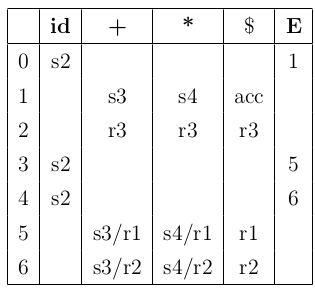
\includegraphics[scale=0.6]{Chapters/Img/c04_12.png}\\
\end{center}

Noto che ci sono dei conflitti, in action [5,+] se voglio favorire l'associativit\'a a sinistra del + scelgo r1, se voglio far valere la precedenza del 
* scelgo s4 per la action[5,*].

\section{More Powerful LR Parsers}
Estendo il parser di prima aggiungendo un simbolo di lookahead; ci sono due metodi:
\begin{itemize}
    \item \textbf{canonical-LR} usa grandi set di items LR(1) per il lookahead \\
    \item \textbf{lookahead-LR o LALR method} basato su set di items LR(0) ed ha pochi stati rispetto ai parsers basati su items LR(1)\\ 
\end{itemize}

\section{Canonical LR(1) items}
Cerco di portarmi dietro pi\'u informazioni, splitto gli stati del SLR. Definisco un \textbf{LR(1) item} come un oggetto della forma 
$[A \rightarrow \alpha\beta ,\ a]$ con a un terminale o un end-marker $\$$ chiamato \textbf{lookahead} dell'item.
Un item $[A \rightarrow \alpha ,\ a]$ viene ridotto solo se il simbolo dopo \'e una a. Il lookahead set dev'essere un subset dei follow di A.

\subsection{Costructing LR(1) sets of Items}
\begin{lstlisting}
    repeat{
        foreach([A -> alpha B beta, a] in I){
            foreach(B -> gamma in P){
                foreach(b in T / b in first(beta alpha))
                    I.add[B -> .gamma, b]
            }
        }
    } until (no more items are added to I)
    return I;
\end{lstlisting}

\subsection{Costructing LR(1) Goto Function}
\begin{lstlisting}
    goto(I,X){
        J = emptySet;
        foreach([A -> alpha X beta, a] in I){
            J.add([A -> alpha X beta, a]);
        }
        return closure(J);
    }
\end{lstlisting}

\subsection{Items(G')}
\begin{lstlisting}
    C = closure({[S' -> .S, $]});
    repeat{
        foreach(set of items I in C){
            foreach(X in V){
                if(goto(I,X) != empty & not in C){
                    C.add(goto(I,X));
                }
            }
        }
    } until(no new sets of items are added to C);
\end{lstlisting}

\subsection{Esempio}
$S' \rightarrow S$\\
$S \rightarrow CC$\\
$C \rightarrow cC|d$\\

Inizio computando la chiusura di $\{ [S' \rightarrow .S,\$ ] \}$ che mi deve matchare con $[A \rightarrow \alpha B \beta,\ a]$ 
($A = S',\ B = S,\ a = \$ $). Devo quindi aggiungere $[B \rightarrow \gamma ,\ b]$ con $b \in first(\beta\alpha)$.
Devo per forza aggiungere $S \rightarrow CC$ e dato che $\beta = varepsilon$, b pu\'o essere solo $\$$.
Quindi aggiungo $[S \rightarrow .CC,\ \$]$.

Continuo la closure con $[C \rightarrow .\gamma ,\ b]$ con $b \in first(C\$) = first(C) = \{ c,\ d \} \implies$ aggiungo gli items 
$[C \rightarrow .cC,\ c],\ [C \rightarrow .cC,\ d],\ [C \rightarrow .d,\ c],\ [C \rightarrow .d,\ d]$; nessuno di questi pu\'o essere 
ulteriormente espanso quindi ho finito per questo set.

$I_0 = \{  [S' \rightarrow .S,\ \$],\ [S \rightarrow .CC,\ \$],\ [C \rightarrow .cC,\ c|d],\ [C \rightarrow .d,\ c|d] \}$\\

Computo $goto(I_0, S)$, devo aggiungere $[S' \rightarrow S.,\ \$]$ che non pu\'o esere ampliato.\\

$I_1 = \{ [S' \rightarrow S.,\ \$] \}$\\

Computo $goto(I_0, C)$ aggiungo $[S \rightarrow C.C,\ \$ ]$ ed espando\\

$I_2 = \{ [S \rightarrow C.C,\ \$],\ [C \rightarrow .cC,\ \$],\ [C \rightarrow .d,\ \$] \}$\\
$I_3 = \{ [C \rightarrow c.C, c|d],\ [C \rightarrow .CC, c|d],\ [C \rightarrow .d, c|d] \}$\\
$I_4 = \{ [C \rightarrow d.,\ c|d] \}$\\

\begin{center}
    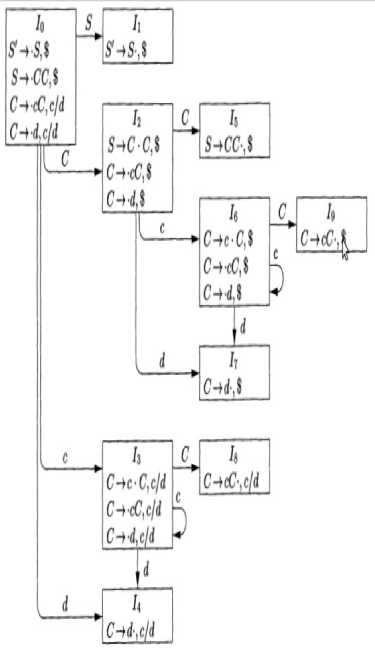
\includegraphics[scale=0.6]{Chapters/Img/c04_13.png}\\
\end{center}

\subsection{Canonical LR(1) Parsing Table}
\begin{itemize}
    \item $C' = \{ I_0,\ I_1,\ ...,\ I_n \}$ la collection dei set LR(1)\\
    \item lo stato i del parser \'e costruito da $I_i$. La parsing action dello stato i \'e determinata:\\
        \item[a)] se $[A \rightarrow \alpha a \beta,\ b] \in I_i$ e $goto(I_i,\ a) = I_j \implies ACTION[i, a] = shift\ j,\ a \in T$ \\
        \item[b)] se $[A \rightarrow \alpha .,\ a] \in I_i, A \not = S' \implies action[i, a] = reduce\ A \rightarrow \alpha '' $\\
        \item[c)] se $[S' \rightarrow S.,\ \$ ] \in I_i \implies action[i, \$] = accept$\\
    \item Se $goto(I_i, A) = I_j \implies goto(i, A) = j$\\
    \item Tutte le entry non definite generano error()\\
    \item Lo stato iniziale \'e costruito a partire da $[S' \rightarrow S, \$]$\\
\end{itemize}

\begin{tcolorbox}\begin{center}
    Se emergono conflitti nella costruzione della parsing table la grammatica \textbf{non \'e LR(1)}.
\end{center}\end{tcolorbox}

\subsection{Esempio}
$S' \rightarrow S$\\
$S \rightarrow CC$\\
$C \rightarrow cC|d$\\

\begin{center}
    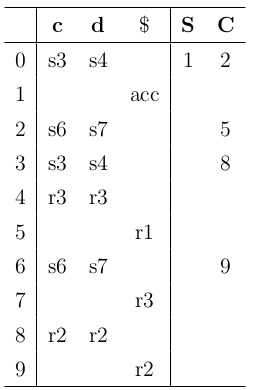
\includegraphics[scale=0.6]{Chapters/Img/c04_14.png}\\
\end{center}

\section{LALR (LookAhead LR) Parsing Table}
\'E spesso usata perch\'e le tabelle LALR sono pi\'u piccole delle canonical LR tables. 

$I_3 = \{ [C \rightarrow c.C,\ c|d],\ [C \rightarrow .cC,\ c|d],\ [C \rightarrow .d,\ c|d] \}$\\
$I_4 = \{ [C \rightarrow .d,\ c|d] \}$\\
$I_6 = \{ [C \rightarrow c.C,\ \$ ],\ [C \rightarrow .cC,\ \$ ],\ [C \rightarrow .d,\ \$ ] \}$\\
$I_7 = \{ [C \rightarrow .d,\ \$ ] \}$\\

Inoltre so che $goto(I_3, c) = I_3,\ goto(I_3,d) = I_4,\ goto(I_6,c)=I_6,\ goto(I_6, d) = I_7$;
in questo caso $I_4$ e $I_7$ hannoun core comune $\{ C \rightarrow .d \}$, $I_3$ ed $I_6$ hanno un core 
$\{ C \rightarrow c.C,\ C\rightarrow .cC,\ C \rightarrow .d \}$.

In generale un \textbf{core} \'e un set di item LR(0) / la grammatica pu\'o produrre pi\'u di due set di item con lo stesso core.

Finch\'e il core di goto(I, X) dipende solo dal core di I, le goto di set mergiati possono essere mergiate. Quindi non ho problemi 
a risolvere la goto di set mergiati. Quindi in pratica se ho una grammatica LR(1) senza conflitti e unisco gli stati con lo stesso core 
potr\'o avere solo conflitti reduce/reduce ed \'e improbabile.

\subsection{LALR Parsing Table}

\begin{itemize}
    \item genero la collection $C = \{ I_0, ...,I_n\}$\\
    \item unisco gli stati in C con la loro unione generando $C' = \{ J_0, ..., J_m \}$ (\textbf{LALR(1) items})\\
    \item genero le action come per cLR su C' (\textbf{LALR(1) collection})\\
    \item Se $I_n \subset J \implies goto(J, X) = gk,\ k = union(item\ LR(1) \ / \ \text{hanno lo stesso core di } goto(I_n, X))$\\
\end{itemize}

\begin{tcolorbox}\begin{center}
    Se emergono conflitti nella costruzione della parsing table la grammatica G \textbf{non \'e LALR(1)}; altrimenti G \'e LALR(1).
\end{center}\end{tcolorbox}

\subsection{Esempio}
$S' \rightarrow S$\\
$S \rightarrow CC$\\
$C \rightarrow cC|d$\\
Ottengo coppie con lo stesso core ($I_3$ e $I_6$, $I_4$ e $I_7$, $I_8$ e $I_9$). Ottengo questa parsing table:

\begin{center}
    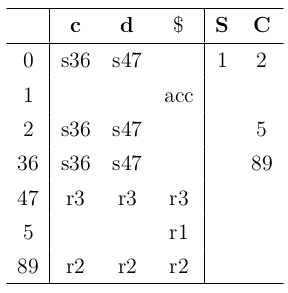
\includegraphics[scale=0.6]{Chapters/Img/c04_15.png}\\
\end{center}

Notare che goto($I_{36}$, C) originariamente era (in LR(1)) $goto(I_3, C) = I_8$ e $I_8$ adesso \'e parte di $I_{89}$, allora 
metto $goto(I_{36}, C) = I_{89}$. 

Naturalmente arrivavo alla stessa conclusione anche per $I_6$, parte di $I_{36}$, con $goto(I_6, C) =  I_9$ che adesso appartiene a $I_{89}$.

Quando parso una stringa i parser LR e LALR fanno le stesse sequenze di riduzioni solo che in LALR hanno nomi diversi. 

\section{Efficient Construction of LALR Parsing Table}
Posso evitare di costruire l'intera collection di LR(1) items; posso rappresentare LR(0) e LR(1) items con il loro \textbf{kernel}
(il body della produzione dopo il punto).
Posso costruire i kernel degli item LALR(1) partendo dai kernel degli item LR(0) per propagazione e spontanea generazione dei lookahead. 
%%%%%%%%%%%%%%%%%%%%%%%%%%%%%%%%%%%%%%%%%%%%%%%%%%%%%%%%%%%%%%%%%%%%%%%%%%%%%%%%%%%%%%%%%%%%%%%%%%%%%%%%%%%%%%%%%%%%%%%%%%%%%%%%%%%%%
%%%%%%%%%%%%%%%%%%%%%%%%%%%%%%%%%%%%%%%%%%%%%%%%%%%%%%%%%%%%%%%%%%%%%%%%%%%%%%%%%%%%%%%%%%%%%%%%%%%%%%%%%%%%%%%%%%%%%%%%%%%%%%%%%%%%%
%%%%%%%%%%%%%%%%%%%%%%%%%%%%%%%%%%%%%%%%%%%%%%%%%%%%%%%%%%%%%%%%%%%%%%%%%%%%%%%%%%%%%%%%%%%%%%%%%%%%%%%%%%%%%%%%%%%%%%%%%%%%%%%%%%%%%
\section{Fine Zampedri}
Ricostruire, se $w \in L(G)$, una rightmost derivation al contrario
%%%%%%%%%%%%%%%%%%%%%%%%%%%%%%%%%%%%%%%%%%%%%%%%%%%%%%%%%%%%%%%%%%%%%%%%%%%%%%%%%%%%%%%%%%%%%%%%%%
\subsection{Esempio}
$S \rightarrow aABe$\\
$A \rightarrow Abc|b$\\
$B \rightarrow d$\\

w = abbcde visto che \'e rightmost devo espandere B dato che \'e il non terminale pi\'u a destra.
$S \rightarrow aABe \rightarrow aAde \rightarrow aAbcde \rightarrow abbcde $\\

\begin{center}
    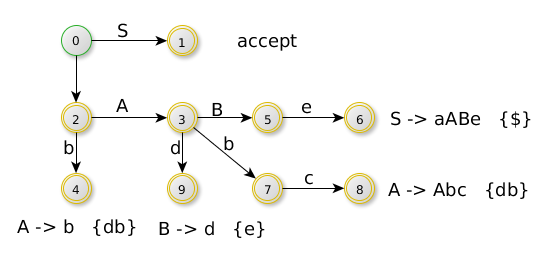
\includegraphics[scale=0.6]{Chapters/Img/c02_14.png}\\
\end{center} 

La sottolineatura significa che se arrivo in questo stato e sto leggendo come prossimo input una d o una b posso fare la riduzione della b usando A. Lo stesso vale per le altre, ovviamente con i loro simboli.
La roba fra parentesi graffe si chiama look-ahead set.

Nel grafo faccio quindi i seguenti passi (i numeri sono i nodi):
\begin{tabular}{ll}
    $0$   &   $abbcde\$$\\
    $0 \rightarrow 2$ consumando \lq $a$ \rq     &  $a || bbcde \$ $\\
    $2 \rightarrow 4$ consumando \lq $b$ \rq     &  $ab || bcde \$ $\\
    4 riduco $A \rightarrow b$  & $aA || bcde$\\
\end{tabular}
A questo punto torno al nodo 2 ovvero il precedente. Vado quindi in 3, perch\'e ho la A al posto della b che avevo prima.\\
torno a 2, vado in 3
\begin{tabular}{ll}
    $3 \rightarrow 7$ consumando \lq $b$ \rq     &  $aAb || cde \$ $\\
    $7 \rightarrow 8$ consumando \lq $c$ \rq     &  $aAbc || de \$ $\\
    8 riduco $A \rightarrow Abc$  & $aA || de$\\
    torno a 7, torno in 3, vado in 9 & \\
    $3 \rightarrow 9$ consumando \lq $d$ \rq     &  $aAd || e \$ $\\
    riduco $B \rightarrow d$ & $aAB || e \$ $\\
    torno a 3, vado in 5, vado in 6 & \\
    $5 \rightarrow 6$ consumando \lq $e$ \rq     &  $aABe || \$ $\\
    6 riduco $S \rightarrow aABe$ & $S || \$ $ \\
    torno a 0, vado in 1, ho finito & \\
\end{tabular}

Noi vogliamo avere grammatiche di tipo LALR(1). Grammatiche: $SLR(1) \subset LALR(1) \subset LR(1)$

\begin{center}
    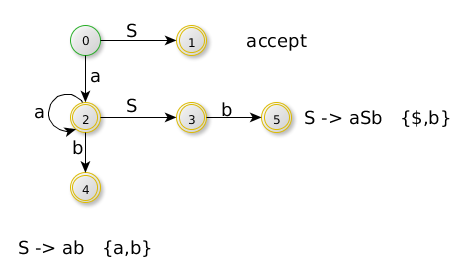
\includegraphics[scale=0.6]{Chapters/Img/c02_15.png}\\
\end{center} 

$S \rightarrow aSb | ab$\\
$w = aaabbb\$$

\begin{tabular}{ll}
    $0$                             &   $aaabbb\$$  \\ 
    $0 \rightarrow 2$               &   $a || aabbb\$$  \\ 
    $2 \rightarrow 2$               &   $aa || abbb\$$  \\ 
    $2 \rightarrow 2$               &   $aaa || bbb\$$  \\ 
    $2 \rightarrow 4$               &   $aaab || bb\$$  \\ 
    4 riduco $S \rightarrow ab$     &    $aaS || bb\$$  \\ 
    torno a 2, vado in 3, vado in 5 & \\
    $3 \rightarrow 5$               &   $aaSb || b\$$  \\ 
    5 riduco $S \rightarrow aSb$    &   $aS || b\$$  \\ 
    torno a 3, vado in 5            & \\
    $3 \rightarrow 5$               &   $aSb || \$$  \\ 
    5 riduco $S \rightarrow aSb$    &   $S || \$$  \\ 
    torno a 0, vado in 1, ho finito & \\
\end{tabular}\\[5pt]

Questa \'e una tabella:\\
\begin{tabular}{|l|l|l|}
    \hline
            &   terminali $\cup\ \$$                                     &   $V \backslash T$     \\
    \hline
    stati   &   shift-k: leggi un simbolo di input e vai allo stato     &   goto-k: descrive le funzioni di transizione  \\
            &   reduce $A \rightarrow b $                               &   identificate dai non terminali quando consumi roba\\
    \hline
\end{tabular}

\section{Algoritmo di shift/reduce}
(comune a SLR(1), LR(1), LALR(1))

\begin{tabular}{ll}
    input   &   w, tabella di parsing bottom-up di tipo $\diamond$, con $\diamond$ scelto fra $\{SLR(1), LALR(1), LR(1)\}$ G.\\
    output  &   derivazione rightmost di w se $w \in L(G)$, altrimenti error()\\  
\end{tabular}

\begin{lstlisting}
    stack.push(s_0);
    buffer = w$;
    while(true){
        let s = stack.top();
        if(M[s,b] == shift-k){
            stack.push(b);
            stack.push(k);
            let b = buffer.readNext(); 
        } else if(M[s,b] == "reduce A -> beta"){
            stack.pop() 2|beta| simboli;
            let j tale che M[m, A] = gj;
            push(A);
            push(j);
            output "A -> beta";
        } else if(M[s,b] = accetta){
            break;
        } else {
            error();
        }
    }
\end{lstlisting}

*sketo*
$S \rightarrow aSb | ab $

\begin{center}
    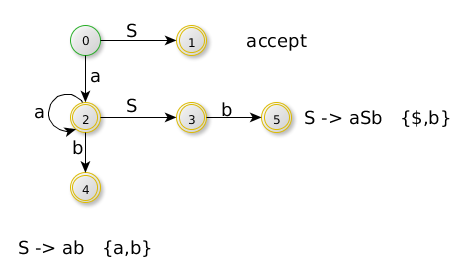
\includegraphics[scale=0.6]{Chapters/Img/c02_15.png}\\
\end{center} 

Questo \'e uguale ma scritto diversamente per separare $\{ \$, b\}$ in $\{4\}$ e $\{b\}$. Nel caso di $w=aaabbb\$$. Una caso rappresenta
il rao pi\'u in alto, mentre l'altro il secondo ramo (pi\'u interno).

\begin{center}
    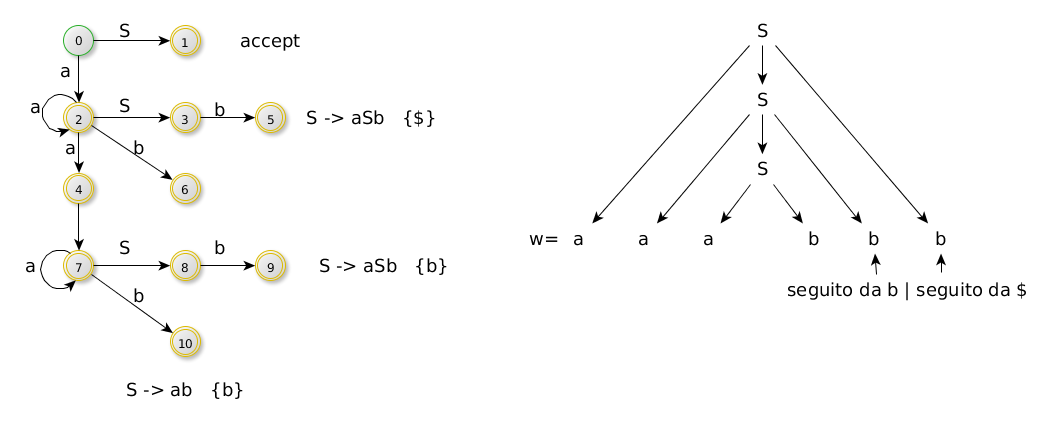
\includegraphics[scale=0.45]{Chapters/Img/c02_16.png}\\
\end{center} 

\begin{itemize}
    \item Automa caratteristico \\
    \item Lookahead Function \\
\end{itemize}

Coppie diverse di questi due insiemi ci danno tipi di grammatiche diverse.

Gli automi che stiamo utilizzando devono essere in grado di ricordare abbastanza da essere in grado di tornare indietro fino al punto 
in cui abbiamo sostituito una certa sequenza di terminali/non terminali con un'altra.

$G = (V,T,S,P)$, aggiungo una produzione $S' \rightarrow S$, $G' = (V \cup \{S'\},T,S',P \cup \{S' \rightarrow S\})$
$A \rightarrow \alpha . \beta $ 

All'inizio ho .S, ovvero non ho ancora letto nulla e devo leggere S.

All'inizio (il nodo iniziale), non ho ancora visto nulla. Visto che S pu\'o iniziare con aSb o ab non sappiamo davanti a quale sviluppo ci troviamo. Il primo stato \'e quindi 

$S' \rightarrow .S$\\
$S \rightarrow .aSb$\\
$S \rightarrow .ab$\\

Questo pu\'o essere visto come un nodo. Da questo stato mi muovo verso un altro stato (con una a-transizione, perch\'e vedo che iniziano 
quasi tutte con a). In questo stato avr\'o:
$S \rightarrow a.Sb$\\
$S \rightarrow a.b$\\

Adesso mi aspetto di vedere l'espansione di una S. Devo quindi aggiungere a questo nodo anche quelle produzioni, e diventa quindi:
$S \rightarrow a.Sb$\\
$S \rightarrow a.b$\\
$S \rightarrow .aSb$\\
$S \rightarrow .ab$\\

Notare che le ultime due sono le stesse delle ultime due del nodo prima. Quella \'e la chiusura, mentre le due prima sono i generatori dello stato (kernel dello stato, \textbf{kernel items}).

Gli stati che sono terminali (ovvero che nol disegno prima avevano le transizioni scritte vicino), sono del tipo $S \rightarrow ab.$ ,
ovvero che hanno incontrato di tutto e di cui si pu\'o eseguire la riduzione. Questi si chiamano \textbf{reducing items}.

Dallo stato con 4 items che avevo prima, si pu\'o fare una b-transizione che va in uno di quelli stati terminali, ovvero:
$S \rightarrow ab.$\\
Questo perch\'e la seconda produzione si aspetta b, che poi completa quello che viene generato da quella produzione.
Sempre da quello stato con 4 produzioni partir\'a anche una a-transizione ed una S-transizione. Per vedere che transizioni devo avere, 
devo vedere la prima lettera dopo il punto per ogni item di quel nodo.

\section{Items}
$G=(V,T,S,P)$\\
$G'=(V \cup \{ S' \},T,S',P \cup \{S' \rightarrow S\})$, con $S' \not\in V$.

Un LR(0)-item di G' \'e una produzione di G con un punto in qualche posizione del body, ovvero $A \rightarrow \alpha . \beta$ .
Alla produzione della forma $A \rightarrow \varepsilon$ corrisponde un solo LR(0)-item, ovvero $A \rightarrow . $\\
L'item $A \rightarrow \alpha . \beta $ \'e detto:
\begin{tabular}{ll}
    iniziale    &   se $A = S' \land \alpha = \varepsilon \land \beta = S$, cio\'e se l'item \'e $S' \rightarrow .S$\\
    accepting   &   se $A = S' \land \alpha = S \land \beta = \varepsilon $, cio\'e se l'item \'e $S' \rightarrow S.$\\
    kernel      &   se \'e un iniziale o tale che $\alpha != \varepsilon$ \\
    closure     &   se $\alpha = \varepsilon$ e non \'e iniziale \\
    reducing    &   se non \'e accepting e $\beta = \varepsilon$, cio\'e se il punto \'e in fondo $\land !accepting$ \\
\end{tabular}
